\documentclass[../main/These_Mathias_Paget.tex]{subfiles}


%----------------------------------------------------------------------------------------
\begin{document}
%----------------------------------------------------------------------------------------

%----------------------------------------------------------------------------------------
\chapter{Coupe de graphe appliquée aux problèmes images}
%----------------------------------------------------------------------------------------

	De nombreux problèmes sont écrits sous la forme d'une énergie multi-label. La reconstruction stéréoscopique par exemple peut s'écrire comme une carte de disparité à optimiser. A chaque pixel est associé un label de disparité prenant des valeurs discrètes dans une intervalle. Nous considérons dans cette partie une énergie multi-label d'ordre 1 de la forme,
	\begin{equation}
	\label{eq:Emulti}
	E(\boldsymbol{l}) = \sum_{p \in \boldsymbol{I}} D_p(l_p) +  \sum_{(p,q) \in \boldsymbol{N'}} R(l_p,l_q)
	\end{equation}
	Nous avons vu qu'une telle peut être optimisée globalement par coupure de graphe. Cependant, cette méthode demande de traiter une graphe volumineux et potentiellement long à optimiser. De plus, cette méthode ne s'applique qu'à une classe de fonction de régularisation réduite. Une méthode approchée est souvent préférée : le problème est décomposé en sous-problèmes binaires, appelés fusion binaire, qui explorent un sous-ensemble de solution. La minimisation successivement de ces sous-problèmes permet de diminuer l’énergie du problème multi-label.

\section{Schéma d'optimisation des problèmes multi-label}
	Pour rappel, la fusion binaire consiste à choisir entre deux valeurs pour chaque valeur d'un vecteur. Les deux propositions de labels sont regroupées dans les vecteurs de label $\boldsymbol{l^1}$ $\boldsymbol{l^2}$. Le vecteur fusionné s'écrit
\begin{equation}
		\boldsymbol{l^{1,2}}_{\boldsymbol{x}} = \boldsymbol{l^1}.\boldsymbol{x} + \boldsymbol{l^2}.\boldsymbol{\bar{x}}
\end{equation}
	où $\boldsymbol{x}$ est un vecteur de variable binaire et l'opérateur point "$.$" est le produit terme à terme. Le problème vise à rechercher l'affectation optimal de $\boldsymbol{x}$. La résolution du problème commence par une initialisation de la solution $\boldsymbol{l^0}$ que nous appellerons solution courante. Le problème est décomposé en sous-problème de fusion selon un schéma d'optimisation qui consiste en un ensemble fini de fusion binaire. La solution courante est remise à jour à chaque résolution d'un problème de fusion en s'assurant que l’énergie est décroissante. Dans le cas où l’énergie est discrète et possède un minimum fini, l'algorithme converge vers une solution. Cette solution n'est pas optimale, les performances d'optimisation dépendent donc de la nature du problème, de l'initialisation, de la stratégie d'exploration de l'espace des solutions et l'optimalité des solutions des sous-problèmes.

\subsection{Garantie de décroissance de l’énergie}

A chaque résolution d'un problème de fusion une nouvelle solution $\boldsymbol{l^*}$ peut être construite. Une condition importante pour la convergence de la méthode est que l’énergie de la solution courante décroît à chaque mise à jour. L'option la plus simple est d'évaluer la nouvelle énergie $E(\boldsymbol{l^*})$ est de remettre à jour la solution courante si
\begin{equation}
		  E(\boldsymbol{l^*}) \leq E(\boldsymbol{l^0})
\end{equation}
Toutefois, pour ces raisons de performance d'optimisation, il est préférable de construire des solutions qui fassent décroître l’énergie. On distingue deux cas, le problème peut être résolue exactement, ou une méthode approchées doit être mise en ouvre.

\subsubsection{Cas Sous-modulaire}

Dans le cas où le problème de fusion est sous-modulaire, le minimum global du problème de fusion peut être trouvé par coupure de graphe avec la structure décrite dans TODO . Si $\boldsymbol{l^0}$ appartient à l'ensemble des fusion $\boldsymbol{l^{1,2}}_{\boldsymbol{x}}$, c'est à dire qu'il existe une affectation de $\boldsymbol{x_0}$ telle que
\begin{equation}
	\boldsymbol{l^{1,2}}_{\boldsymbol{x_0}} = \boldsymbol{l^0}
\end{equation}
alors la solution obtenu $\boldsymbol{l^*}$ est nécessairement d’énergie inférieure à la solution courante,
\begin{equation}
	\min_{\boldsymbol{x}}{E(\boldsymbol{l^{1,2}}_{\boldsymbol{x}})} \leq E(\boldsymbol{l^0})
\end{equation}
Le fait d’obtenir le minimum global du sous-problème permet d'avoir une décroissance rapide de l’énergie.

\subsubsection{Fusions approchées}

	Soit $F(\boldsymbol{x})$ la fonction qui décrit l’énergie des solution fusionnées, la contrainte de sous-modularité sur la fonction $F$ limite le choix de la fonction de régularisation selon le type de fusion choisi. Ainsi une fonction utilisée fréquemment comme la fonction quadratique tronquée ne s'écrit pas comme un problème de fusion sous-modulaire dans les fusions décrites dans la partie~\ref{ss:s_mod_form}. Une approche simple est de limiter l'opération de fusion à un sous-ensemble de label de sorte que le problème devienne sous-modulaire. Cette méthode s'appelle fusion partielle.
	
	Une autre solution est de relaxer le problème en ajoutant une fonction $F'$ à valeur positive afin de rendre la fonction $F$ sous-modulaire. Soit $\boldsymbol{x^0}$ l'affectation qui donne les labels $\boldsymbol{l^0}$, si $F'(\boldsymbol{x^0})=0$ alors optimiser $F+F'$ permet de réduire l’énergie,
	\begin{equation}
	\min_{\boldsymbol{x}}{F(\boldsymbol{x})} \leq \min_{\boldsymbol{x}}{( F(\boldsymbol{x}) + F'(\boldsymbol{x}) )} \leq F(\boldsymbol{x^0})
	\end{equation}
La solution trouvée est donc une solution optimale du problème relaxé. Cela limite l’efficacité de l'optimisation, mais ces techniques peuvent être suffisantes pour résoudre des problèmes avec peu de termes non-sous-modulaires et de faible amplitude, où l'utilisation de méthode plus complexe ne se justifie pas. La fonction $F'$ qui impacte le moins la solution du problème est celle qui annule les termes quadratiques là où $F$ n'est pas sous-modulaire. Cette méthode sera dénommé "fusion relaxée" dans la suite du manuscrit. La fusion partielle décrite dans le paragraphe précédent peut être vu comme un cas particulier où $F'$ est une fonction qui interdit le changement de certaines variables.
	
	Enfin la méthode $QPBO$ peut être mise en ouvre. La solution partielle issue de l'optimisation garantit de diminuer l’énergie du fait de la propriété d'autarcie. L'optimalité de la solution peut être améliorée à l'aide d'une des heuristiques proposées. Cette approche est adaptée aux fonctions fortement non-sous-modulaires, toutefois elle plus volumineuse (deux fois plus de variables) et coûteuse en calcul pour une résolution du problème éventuellement peu complète. Il y a donc un enjeu à écrire autant que possible les problèmes sous la forme d'une fonction sous-modulaire pour une meilleur optimisation.

\subsection{Schémas avec fusions binaires sous-modulaires}
\label{ss:s_mod_form}

Pour certaines catégories de fonction, le problème de fusion peut être écrite à l'aide d'une fonction sous-modulaire. Elle peuvent d'appliquer à toute fusion dans le cas convexe (Partie~\ref{sss:fus_conv}. Pour des cas particuliers de fusion, d'autres type de fonctions de régularisation peuvent être utilisées (Partie~\ref{sss:swap} et Partie~\ref{sss:alp_exp}).

\subsubsection{Fusion Convexe}
\label{sss:fus_conv}
	Dans un cas où la régularisation est une fonction convexe de la différence des labels, un échange de variable particulier permet de rendre $F$ sous-modulaire. Plutôt que de prendre le problème de fusion $(\boldsymbol{l^1},\boldsymbol{l^2})$, on traite le problème de fusion $(\boldsymbol{l^{min}},\boldsymbol{l^{max}})$ avec $\boldsymbol{l^{min}}= \boldsymbol{l^1} \vee \boldsymbol{l^2}$, $\boldsymbol{l^{max}}= \boldsymbol{l^1} \wedge \boldsymbol{l^2}$, $\vee$ (ou $\wedge$) le minimum (ou le maximum) terme à terme.  La condition de sous modularité devient
	\begin{equation}
	\label{eq:cond_conv}
	R(l^{min}_i,l^{min}_j) + R(l^{max}_i,l^{max}_j) \leq R(l^{min}_i,l^{max}_j) + R(l^{max}_i,l^{min}_j)	
	\end{equation}
	Soit le vecteur de différence de label $\boldsymbol{dl} = \boldsymbol{l^{max}}-\boldsymbol{l^{min}}$, ces composantes sont par définition positives. Si on considère que la fonction de régularisation ne dépends que de la différence de label $k$, alors la condition devient
	\begin{equation}
	\label{eq:f_conv}
	r(k) + r(k-dli+dl_j) \leq r(k-dl_i) + r(k+dl_j)
	\end{equation}
	Si la fonction est $r$ est convexe par définition,
	\begin{equation}
	\label{eq:f_conv2}
		\begin{aligned}
	r(k) & \leq \frac{dl_j}{dl_i+dl_j} r(k-dl_i) + \frac{dl_i}{dl_i+dl_j} r(k+dl_j) \\
	r(k-dl_i+dl_j) & \leq \frac{dl_i}{dl_i+dl_j} r(k-dl_i) + \frac{dl_j}{dl_i+dl_j} r(k+dl_j)
		\end{aligned}
	\end{equation}
	en sommant les deux inégalités \ref{eq:f_conv2}, on retrouve l'inégalité \ref{eq:f_conv}. Ainsi toute fusion binaire avec une fonction de régularisation de la différence de label convexe s'écrit sous la forme d'une $FPB$ quadratique sous-modulaire et peut être minimisée par coupure de graphe.

\subsubsection{$\alpha$-$\beta$-Échange}
\label{sss:swap}
Deux fusions, le ré-étiquetage et échange de label, permettent d'optimiser la majorité des fonction de régularisation. La fusion ré-étiquetage consiste à proposer pour tous les labels $\alpha$ de la solution courante, le label $\beta$, et le reste de la solution est inchangée. L'échange d'étiquette (\cite{Veksler99t}) consiste à réaliser simultanément un ré-étiquetage $\alpha/\beta$ et $\beta/\alpha$. Par changement de variable, l'échange d'étiquette peut s'écrire comme un ré-étiquetage : les labels $\alpha$ sont transférés dans une solution et les labels $\beta$ dans l'autre. La condition de sous-modularité sur la fonction de régularisation pour ces deux fusions sur la fonction de régularisation est,
	\begin{equation}
	\label{eq:reet}
	R(\alpha,\alpha) + R(\beta,\beta) \leq R(\beta,\alpha) + R(\alpha,\beta)	
	\end{equation}
	et pour une fonction de régularisation $r$ de la différence de label,
	\begin{equation}
	\label{eq:reet2}
	2r(0) \leq r(\beta-\alpha) + r(\alpha-\beta)	
	\end{equation}
	Il suffit que la fonction $r$ soit nulle en zéro et positive pour que le problème soit sous-modulaire. Cette condition est respectée par la majorité des fonctions de régularisation ce qui permet de la mettre en œuvre l’échange de label pour presque tous les problèmes. Le schéma $\alpha$-$\beta$-Échange consiste à réaliser successivement l'ensemble des échanges paramétrés par $(\alpha,\beta) \in L^2$. Le nombre de fusion binaire à réaliser peut être important, et comme seul une partie de l'image est remise en jeu, les performances d'optimisation sont limitées.

\subsubsection{$\alpha$-Expansion}
\label{sss:alp_exp}

La fusion expansion (\cite{Veksler99t}) consiste à proposer le label $\alpha$ pour touts les labels. La contrainte de sous-modularité sur la fonction de régularisation devient,
	\begin{equation}
	R(l_i,l_j) + R(\alpha,\alpha) \leq R(l_i,\alpha) + R(\alpha,l_2)	
	\end{equation}
	Si $R(\alpha,\alpha)=0$ alors $R$ est une distance. La condition sur la fonction $r$ de la différence de label est
	\begin{equation}
	r(l_i-l_j) + r(0) \leq r(l_i-\alpha) + r(\alpha-l_2)	
	\end{equation}
	Si $r(0)=0$, la fonction $r$ est sous-additive. Une condition suffisante sur $r$ est concave et croissante sur $\mathbb{R}^+$ ainsi que concave et décroissante sur $\mathbb{R}^-$. L’avantage de l'expansion est que la proposition de label est indépendante de la solution courant et que cette proposition respecte l'a priori fronto-parallèle. Si la solution est constante par morceaux, ce sont des pans entiers de solution qui sont proposés lors de la fusion.
	Le schéma d'optimisation  $\alpha$-Expansion consiste à réaliser successivement l'ensemble des expansion paramétrée par $\alpha \in L$. Ces fusions peuvent être pris dans un ordre croissant ou dans un ordre aléatoire. Cette méthode a montré des résultats intéressants pour de nombreux problèmes, où l'approximation de la solution est bonne pour un temps de calcul raisonnable.

\begin{table}
\begin{center}
\begin{tabular}{c|cc}
\hline
Nom & $\boldsymbol{l^1}$ & $\boldsymbol{l^2}$ \\
\hline
Ré-étiquetage & $l_{i}^{0}$ &  $\left\{\begin{array}{cc} \beta & si\:l_{i}^{0}=\alpha  \\  l_{i}^{0} & sinon \end{array}  \right. $ \\
Échange & $\left\{\begin{array}{cc} \alpha & si\:l_{i}^{0}=\beta  \\  l_{i}^{0} & sinon \end{array}  \right. $ &  $\left\{\begin{array}{cc} \beta & si\:l_{i}^{0}=\alpha  \\  l_{i}^{0} & sinon \end{array}  \right. $ \\ 
Expansion & $l_{i}^{0}$ & $\alpha$ \\
Saut & $l_{i}^{0}$ & $l_{i}^{0}+\delta$ \\
%Flou & $l_{i}^{0}$ & $l_{i}^{0:flou}$ \\
%Bruit & $l_{i}^{0}$ &  $l_{i}^{0} + bruit$ \\
\end{tabular}
\end{center}
\caption{Proposition de label pour les différentes fusions}
\label{tab:fusion}
\end{table}

\subsection{Schéma d'optimisation par résolution approchée}

Il n'est pas toujours possible de trouver une écriture des fusions qui puisse être optimisée globalement. Ainsi, des schémas d'optimisation approchée ont été proposé. Ils ont été proposés dans le contexte de fonctions de régularisation particulières, convexes seulement autour de zéro (Parties~\ref{sss:anna}~et~\ref{sss:ICIP1}. D'autres schéma ont été proposés notamment pour traiter les problèmes issus d'un réduction d'ordre potentiellement fortement non-sous-modulaires.

\subsubsection{$\alpha$-Expansion Quantifiée}
	\label{sss:anna}
	Cette méthode introduite par \cite{Jezierska11CVPR} s'applique à des fonctions de régularisation convexes tronquée. Autour de zéro la fonction est convexe, et au delà d'un seuil $T$ sur la différence de label, la fonction est constante. Le schéma d'optimisation est composé d'$\alpha$-expansion partiels appelé "Fusion quantifiée" et de sauts. Les "Fusion quantifiée" de paramètre $\alpha$-$T$ sont des expansions limitées aux labels dont les valeurs sont en dehors de l'intervalle $[\alpha-T,\alpha +T]$. La fusion ainsi définit possède une écriture sous-modulaire. Les fusion quantifiée sont réalisée à un intervalle de valeur $T$. Les valeurs intermédiaire sont obtenue en appliquant des sauts décrit ci-après. La fonction de régularisation n'étant pas convexe, le problème de saut n'est pas sous-modulaire. Les auteurs choisissent de résoudre le problème avec une approximation convexe de la fonction de régularisation et de rejeter cette solution si cette solution augmente l’énergie du problème initial.
	
	% TODO : illustration d'une fonction tronquée
	
\paragraph*{Saut}
	Le saut consiste à fusionner la solution courante avec la solution plus une constante $\delta$ sur chaque label. La condition sur $R$ devient
	\begin{equation}
	R(l_i,l_j) + R(l_i+\delta,l_j+\delta) \leq R(l_i,l_j+\delta) + R(l1+\delta,l_2)	
	\end{equation}
Cette fusion explore localement l'énergie autour la solution. L’énergie multi-label étant souvent non-convexe, elle possède souvent de nombreux minima locaux, ainsi cette fusion n'est pas adaptée lorsque la solution est très éloignée de la solution minimale. Le problème s'écrit sous la forme d'une fusion convexe (Partie~\ref{sss:fus_conv}) avec les même contraintes sur la fonction de régularisation.

\subsubsection{Expansion-Saut alternés}
	\label{sss:ICIP1}

	Dans \cite{Paget15ICIP}, nous proposons d'alterner des $\alpha$-expansion avec des sauts à plusieurs pas. L'objectif est de pouvoir traiter des fonctions convexes autour de zéros et concave pour des grandes valeurs. Ces deux fusions utilisée sont complémentaires : la première est sous-modulaire dans la partie concave de la fonction, et le seconde dans la partie convexe. Dans l'article, les non-sous-modularité sont gérées en restreignant les labels mis en jeu dans la fusion. Dans le manuscrit, nous utilisons la fusion relaxée.

\subsubsection{Autres schémas}

	\paragraph*{LogCut}
	%D'autre fusion ont pu être proposées,
	Les labels peuvent être écrit en base 2 de sorte que chaque label est écrit comme une chaîne de de $0$ et de $1$. Le problème est d'optimiser les valeurs de bits de la solution. Le nombre de variable par label est en $\text{ln}_{2}$ du nombre de valeur de label, c'est donc une écriture plus compact que le problème décrit dans TODO . Toutefois, l'ordre de la fonction pseudo-booléenne peut être très élevé : dans le cas d'un maximum de vraisemblance l'ordre de la $FPB$ est aussi en $\text{ln}_{2}$ du nombre de valeur de label.\cite{Lempitsky10PAMI} propose de ne remettre en jeu qu'un bit par label à la fois. L'auteur propose d'ajouter une constante au label avant de la convertir en base 2 afin d'explorer d'autres valeur de label.
De plus l'auteur propose de réaliser les fusions en parallèle plutôt que successivement. $n$ branches sont traitée en parallèles réalisant chacun un sous-ensemble des expansions. Les résultats des $n$ branches sont alors fusionnés deux à deux. La sous-modularité du problème de fusion des branches n'est pas garantie, des méthodes approchées sont mises en œuvre.

	\paragraph*{Bruit-Flou}
	\cite{Ishikawa11PAMI} propose deux fusions : la fusion avec un bruit et la fusion avec la solution floutée. La fusion avec un bruit permet d’explorer de manière aléatoire l'espace des solutions. L’inconvenant de cette méthode est que la proposition faite possède une énergie de régularisation élevée du fait de l'absence de structure. Ainsi les solutions fusionnées ont tendance elles-aussi d'avoir des valeurs élevées. La fusion par une solution floutée permet de proposer une version plus lisse de la solution courante. Le schéma d'optimisation alterne des fusions Flou et des fusions Bruité. Un tel schéma est adapté aux problèmes d'ordre élevé. Ce schéma est utiliser pour minimiser des fonctions issue d'une réduction d'ordre qui possède souvent des termes de nombreux terme non-sous-modulaires et des variables additionnelles. Ces variable n'ont pas d'interprétation en terme d'image de sorte que des fusions Expansion et Saut ne sont pas forcement pertinents.

\section{Application au dé-bruitage}

Le problème de dé-bruitage et les résultats sont présentés dans cette partie afin d’illustrer un cas de traitement d'image où le modèle des données est parfaitement connue.

\subsection{Modélisation du problème}
	Le dé-bruitage est un cas particulier de restauration d'image. Il s'agit de reconstruire à partir d'une image, décrit par le vecteur de label $\boldsymbol{l^b}$ soumise à un bruit d'estimer une image $\boldsymbol{\hat{l}}$ aussi proche possible de l'image originale $\boldsymbol{\dot{l}}$. En faisant l'hypothèse que la perturbation est un bruit additif,  $\boldsymbol{l^b} = \boldsymbol{\dot{l}} {+}  \boldsymbol{B}, \;
 \boldsymbol{B} \sim \mathbb{P}_b(\boldsymbol{B})$, le terme de vraisemblance est égale à la distribution du bruit $\mathbb{P}(\boldsymbol{\dot{l}} | \boldsymbol{l^b}) = \mathbb{P}_b(\boldsymbol{l^b}  {-} \boldsymbol{\dot{l}})$. Dans le cas d'un bruit centré, la solution par maximum de vraisemblance est $\boldsymbol{\hat{l}}_{ML} = \boldsymbol{l^b}$, c'est à dire qu'aucun traitement n'a été appliqué à l'image. Il est donc nécessaire d'introduire un a priori sur la solution pour espérer séparer le bruit du signal. L'a priori sur la solution doit décrire les caractéristiques recherchées de la solution. L'a priori utilisé est que deux pixels voisins dans l'image ont une valeur égale. Nous faisons l'hypothèse que l'écart des valeurs entre deux pixels voisins suit une loi $l_i-l_j \sim E $, cette loi étant la même sur toute l'image et que le bruit sur chaque pixel est indépendant. Le $-\text{log}$ de la probabilité a posteriori est alors
\begin{equation}
\begin{aligned}
E(\boldsymbol{l}) &= \sum_{i \in \boldsymbol{I}}{ f(l^b_i - l_i)} + 
\lambda \sum_{(i,j) \in \boldsymbol{N'}}{ g(l_i-l_j) }
\end{aligned}
\end{equation} 
où $f$ est le $-\text{log}$ de la distribution du bruit et $g$ le $-\text{log}$ de la distribution de l’écart de valeur entre des pixels voisins. Le paramètre $\lambda$ est un paramètre additionnel qui permet de régler l'intensité de la régularisation. Dans la pratique il est nécessaire de régler ce paramètre pour arriver au compromis désiré entre attache aux données et régularisation. Ces fonctions peuvent être définies à une constante près sans modifier la solution du problème, nous prendrons $f(0)=0$ et $g(0)=0$. Toutes les valeurs manipulées dans les graphes sont entières, ainsi les valeurs des fonctions sont quantifiées. Dans cette partie, nous utiliserons des images test fréquentes dans la littérature, il s'agit des images en niveau de gris Lena, Pepper, Barbra, Boat et House représentées dans la Figure~\ref{fig:denoise_base}. La Figure~\ref{fig:lena} représente l'image Lena originale et l'image bruitée, ainsi qu'un agrandissement sur une zone d'intérêt.

\begin{figure}
\centering
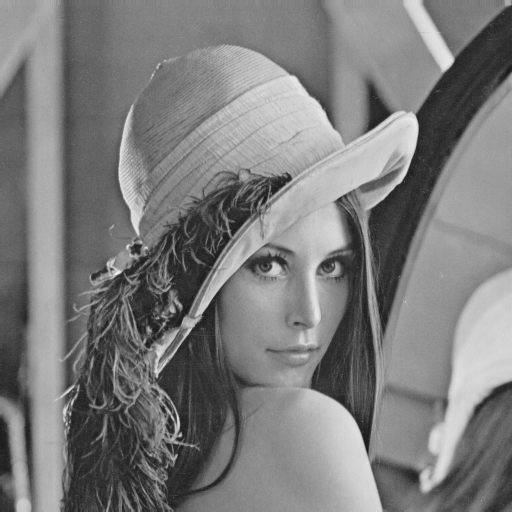
\includegraphics[scale=0.3]{Images/2_ref}
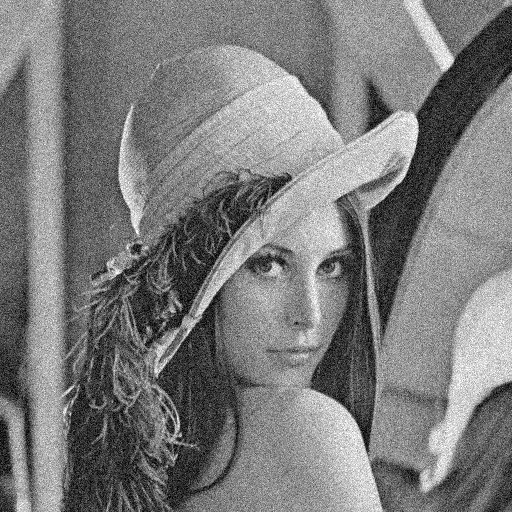
\includegraphics[scale=0.3]{Images/2_noisy}
\hspace{10 pt}
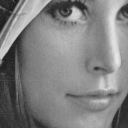
\includegraphics[scale=1.2]{Images/2_ref_}
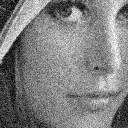
\includegraphics[scale=1.2]{Images/2_noisy_}
\caption{Image originale et image bruitée (bruit gaussien indépendent d'écart-type $\sigma=20$ et agrandissements centrés sur une zone d’intérêt}
\label{fig:lena}
\end{figure}

\begin{figure}
\centering
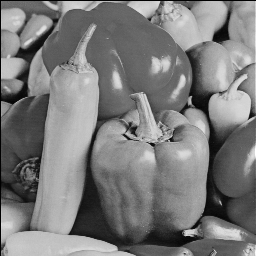
\includegraphics[scale=0.4]{Images/2_pepper}
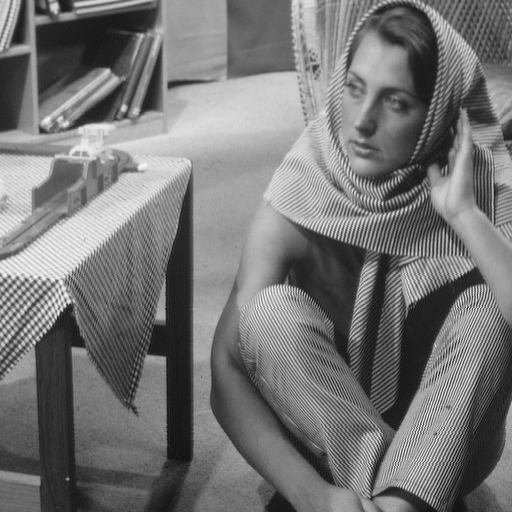
\includegraphics[scale=0.2]{Images/2_barbra}
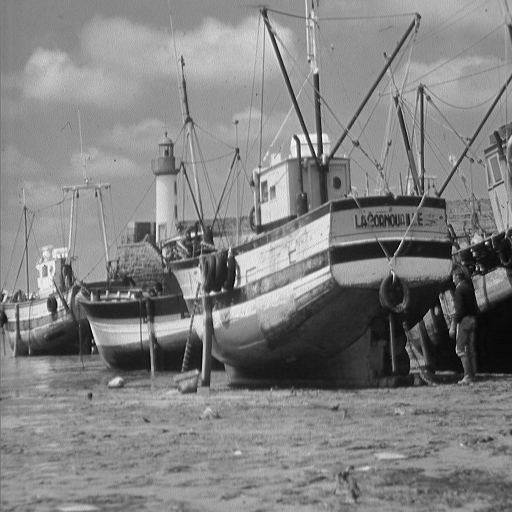
\includegraphics[scale=0.2]{Images/2_boat}
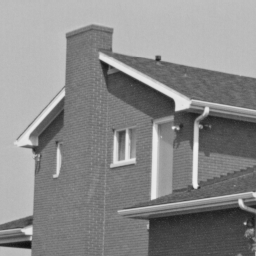
\includegraphics[scale=0.4]{Images/2_house}
\caption{La base de test est composé de l'image Lena et des quatres images ci-dessus. De gauche à droite : Pepper, Barbra, Boat, House.}
\label{fig:denoise_base}
\end{figure}

\subsection{Comparaison des fonctions de régularisation}

Le choix de la fonction de régularisation a un impact fort sur la forme de la solution obtenue. Nous étudions dans un premier temps les résultats issus de régularisation convexe (Partie~\ref{sss:comp_reg_conv}). Nous illustrerons l'effet de certaines caractéristiques de la fonction de régularisation sur le résultat (Partie~\ref{sss:sub_add}). Nous proposons une méthode pour rendre les solutions de différents comparables entre elle en terme d'intensité de la régularisation(Partie~\ref{sss:normalize_energy}).

\subsubsection{Comparaison norme L2, norme L1, "norme L1 lissée"}
\label{sss:comp_reg_conv}

Un des premiers modèles en traitement d'image est le modèle de Tikhonov avec une attache aux données $L2$ et une régularisation $L2$. Ce modèle est quadratique et il est simple à optimiser par méthode continue. Le problème d'un tel modèle est que la solution est une version floutée de l'entrée et ne conserve pas les contours. Plus tard, la normalisation par la norme $L1$ a été introduite. Ce modèle possède des propriétés de parcimonie : La solution à tendance favoriser des solutions constantes par morceaux et ainsi les contours sont préservés. Ce modèle est simple à optimiser par coupure de graphe. L’inconvénient est que ce modèle s'adapte mal à des variations lentes de l'intensité qui sont fréquentes dans les images. Il en résulte un effet de marche d'escalier dans ces zones. Ce problème peut être résolue en introduisant un version lissé de la norme $L1$, possédant une cuvette convexe autour de zéro analogue à la norme $L2$. La Figure~\ref{fig:L1_L2} présente les résultats pour les trois modèles sur l'image Lena. Dans le cas de la norme $L2$, la solution est flou et les contours ne sont pas préservés. Dans le cas de la norme $L1$, les contours sont conservés ( sur le nez et l'œil par exemple) mais un effet de marche d'escale apparaît dans les zones de dégradé lent (la joue par exemple). La solution avec la "norme $L1$ lissée" a ces contours préservé et des variations progressives de l'intensité dans les zones de dégradé.

\begin{figure}
\centering
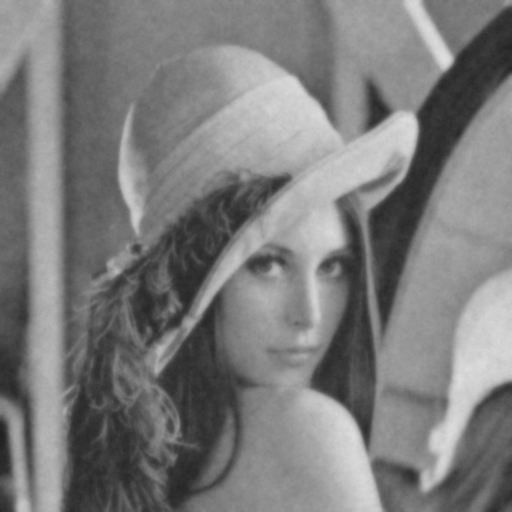
\includegraphics[scale=0.25]{Images/2_gauss}
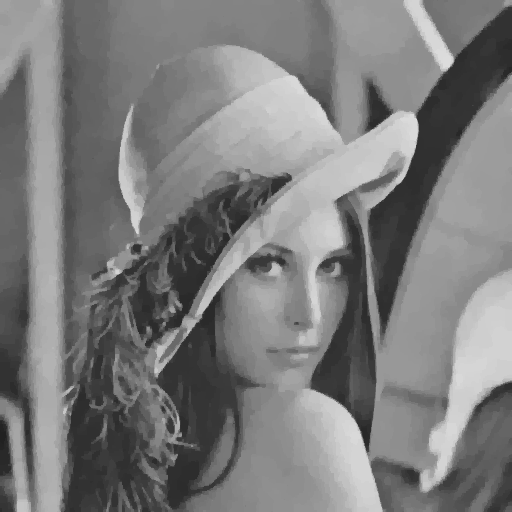
\includegraphics[scale=0.25]{Images/2_1}
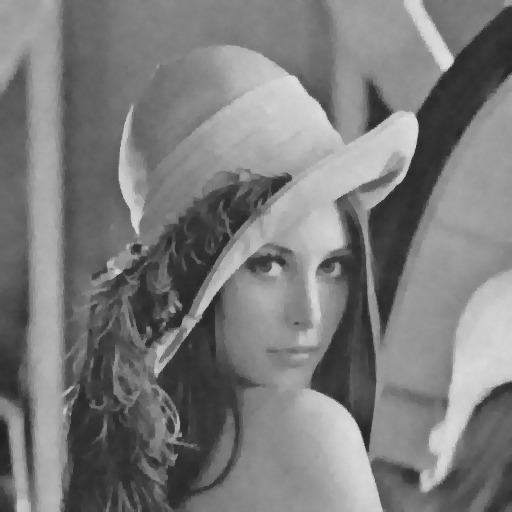
\includegraphics[scale=0.25]{Images/2_2}
\hspace{10 pt}
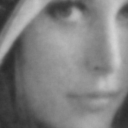
\includegraphics[scale=1]{Images/2_gauss_}
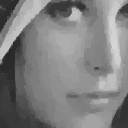
\includegraphics[scale=1]{Images/2_1_}
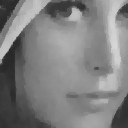
\includegraphics[scale=1]{Images/2_2_}
\caption{Résultat de dé-bruitage de l'image Lena avec un régularisation par la norme $L2$ (première colonne),la norme $L1$ et la "norme $L1$-lissée". Sur la deuxième ligne, un agrandissement de la solution. Nous remarquons l'effet d'escalier dans le cas de la norme $L1$ sur la joie de Lena, cet effet n'est plus visible dans le cas de la "norme $L1$-lissée".}
\label{fig:L1_L2}
\end{figure}

Les modèles convexes peuvent donner des solutions satisfaisantes cependant les modèles non-convexe sont fréquents. En effet certaines propriétés recherchées ne peuvent pas être trouvées dans la familles des fonctions convexes.

\subsubsection{Sous-additivité et sur-additivité des fonctions de régularisation}
\label{sss:sub_add}

La sous-additivité de la fonction $f$ s'écrit
\begin{equation}
f(x+y) \leq f(x) + f(y)
\label{eq:sub_add}
\end{equation}
de même la super-additivité de la fonction $f$ s'écrit
 \begin{equation}
f(x) + f(y) \leq f(x+y)
\label{eq:sup_add}
\end{equation}
Dans le cas où $f$ est une fonction qui donne le coût en fonction de l'erreur avec $f(0)=0$, il est préférable de regrouper les erreurs si $f$ est sous-additive, et répartir l'erreur si $f$ est super-additive. Considérons maintenant $f$ un fonction symétrique et croissante sur $\mathbb{R}^{+}$, si $x$ est $y$ sont de signe opposés, alors la fonction est sous-additive. Ainsi les fonctions $f$ ont tendance à diminuer l'amplitude de l'erreur lorsqu'elle est de signe différent. Si $x$ et $y$ sont de même signe, on distingue deux cas :
\begin{itemize}
\item $f$ est concave sur $\mathbb{R}^{+}$. Alors $f$ est sous-additive. Regrouper l'erreur fait diminuer l’énergie.
\item $f$ est convexe sur $\mathbb{R}^{+}$. Alors $f$ est super-additive. Répartir l'erreur fait diminuer le coût.
\end{itemize}
En présence d'un contour entre deux plateaux à des valeurs différentes, la transition de se fera de manière différente en fonction de la forme de $f$. Dans le cas d'une fonction convexe, la transition sera progressive.  Avec une fonction concave, un transition rapide sera privilégiée et ainsi, les fonctions concaves conservent les contours. Les dégradés progressifs sont bien reconstruits avec des fonctions convexes mais un effet de marche d'escalier peut apparaître avec les fonctions concave. La norme $L1$ est un cas limite car elle est à la fois concave et convexe sur $\mathbb{R}^{+}$ : les relations (\ref{eq:sub_add}) et (\ref{eq:sub_add}) deviennent des égalité. Il existe donc de nombreuses configurations avec un coût équivalent. En pratique, les méthodes d'optimisation ont tendance à sélectionner des solutions parcimonieuses parmi l'ensemble des solutions et donc décrivent mal les dégradés dans l'images.
	
\begin{figure}
\centering
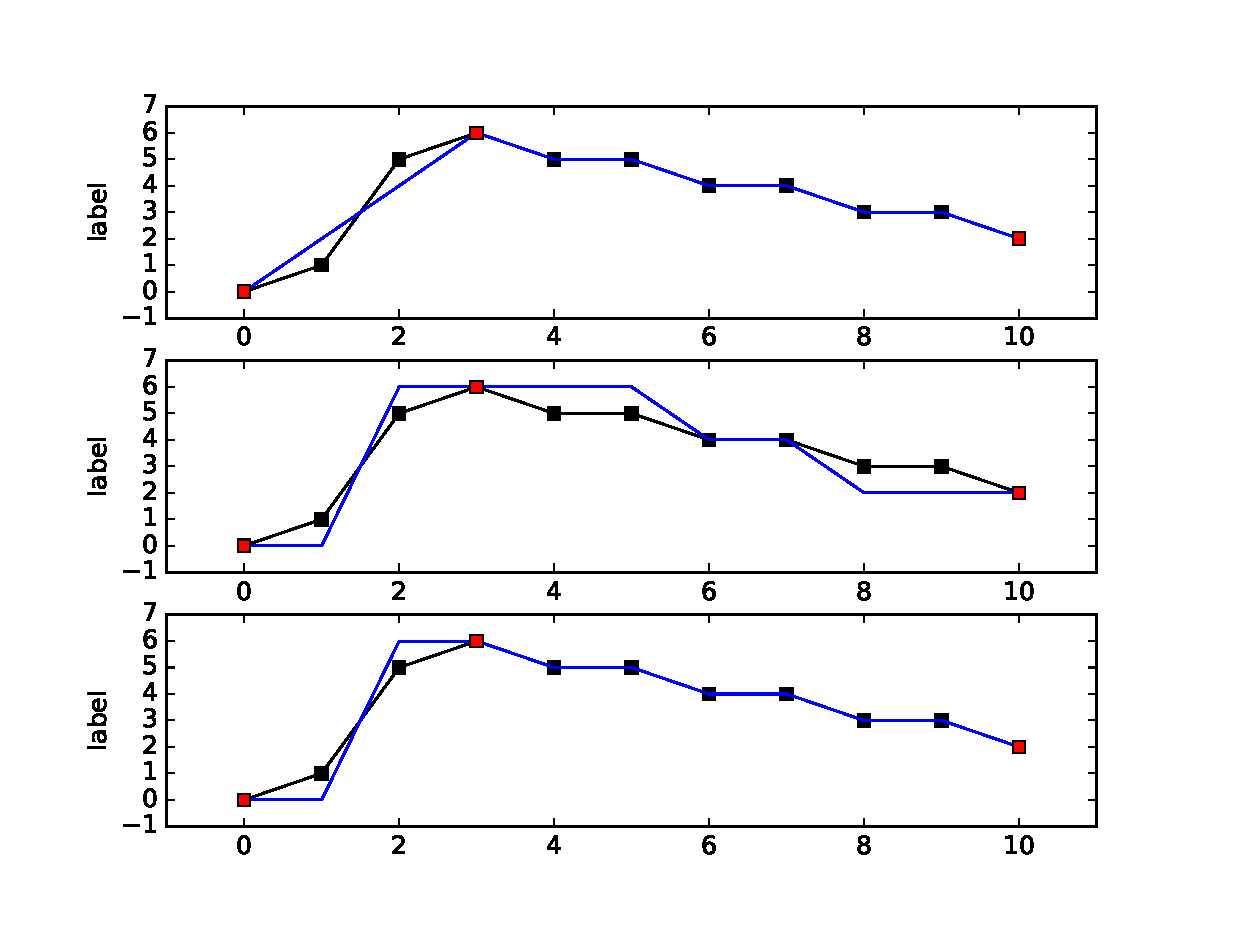
\includegraphics[scale=0.7]{Data/SEF_comp}
\caption{Comparaison des résultats de dé-bruitage du signal  pour trois modèles. Le signal est représenté en noir, les valeurs en rouge sont fixées et ne sont pas mise en jeu dans l'optimisation. La solution optimale est représenté en bleu. La fonction d’attache au données est $f(x)=x^2$ pour les trois modèle. La fonction de régularisation est respectivement $g_1(x)=2x^2$, $g_2(x)=4\sqrt{|x|}$ et $g_3 = 10SEF_{-2,2}(x)$. Ces fonction sont représentées dans la Figure~\ref{fig:comp_opt_} Dans le première modèle, en haut, la fonction convexe donne une solution très lisse où le contour entre $x=0$ et $x=2$ est lissé. Dans deuxième modèle, au milieu, la fonction concave donne une solution constante par morceaux avec des ruptures nettes. Les contours sont préservés mais l'effet de marche d'escalier apparaît dans les zones de dégradé entre $x=4$ et $x=10$. Dans le dernier modèle, en bas, la forme de la fonction de régularisation permet à la fois de préserver les contours et de suivre les dégradés progressifs.}
\label{fig:comp_opt}
\end{figure}

Une solution pour éviter l'effet de marche d'escalier tout en conservant les contours est d'utiliser des fonctions convexe autours de zéro, relativement lisse, et concave pour des plus grandes valeurs. On trouve dans cette catégorie la norme $L2$ tronquée, la norme "$L1$-lissée" et la famille des exponentielles lissée $SEF$ pour un paramètre de forme inférieur à $1$. Les $SEF$ sont paramétré par $a$ la forme, et $s$ l’échelle,
\begin{equation}
SEF_{a,s}(x) =  \frac{ \left( 1+(x/s)^2 \right)^{a/2} - 1}{a/2}
\label{eq:def_SEF}
\end{equation}
Pour $a=2$, $SEF$ est une fonction quadratique. Ces fonctions ont la particularité d'être une approximation quadratique autour de zéro et une puissance pour de grandes valeurs. L'intérêt de telles fonctions sont illustrées dans les Figures~\ref{fig:comp_opt}~et~\ref{fig:comp_opt_}. Elles permettent d'obtenir des solutions qui présentent des dégradées progressifs et des contours nets.

\begin{figure}
\centering
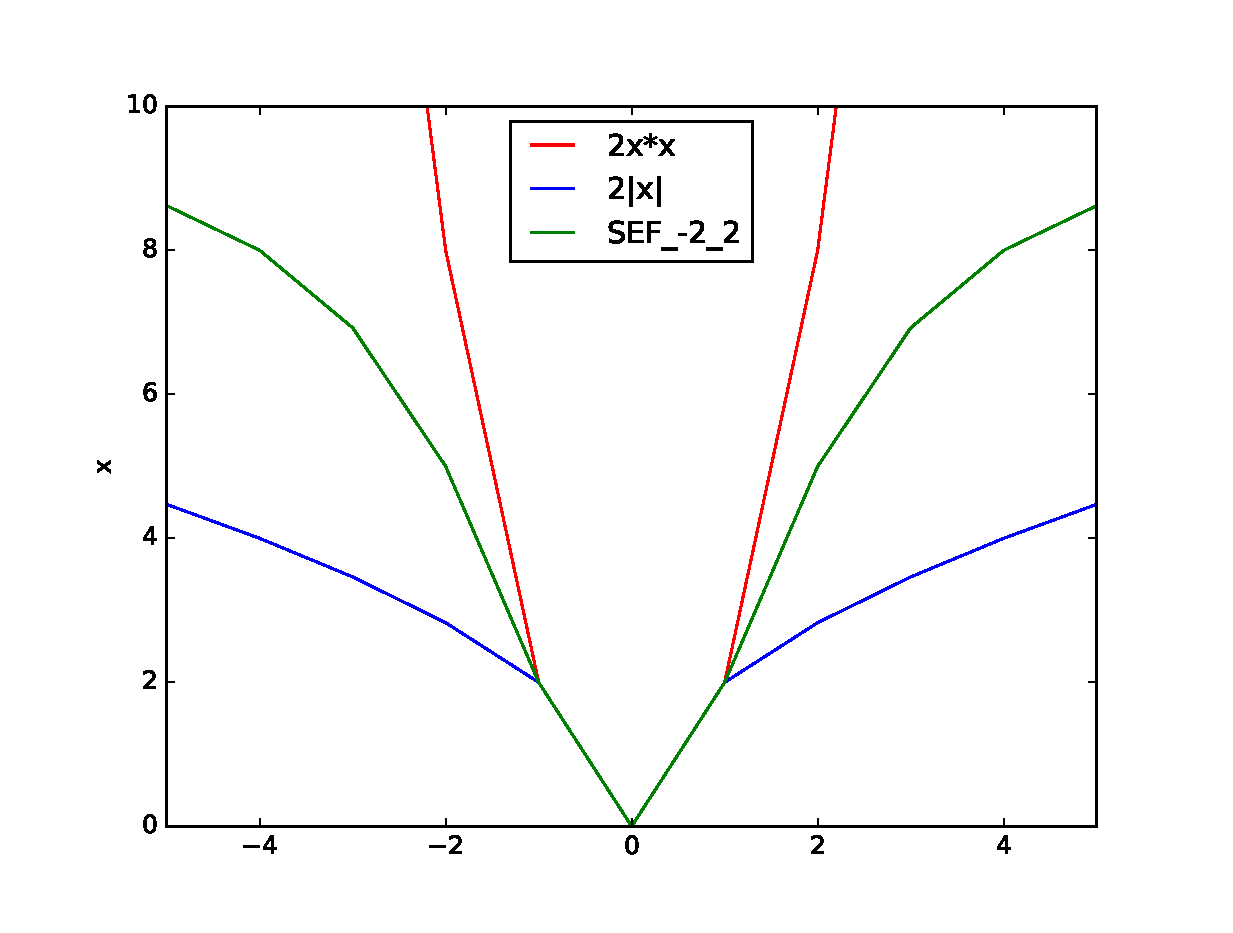
\includegraphics[scale=0.6]{Data/fcn}
\caption{Fonctions de régularisation utilisé dans l'exemple de la Figure\ref{fig:comp_opt}}
\label{fig:comp_opt_}
\end{figure}

\subsubsection{Réglage du paramètre de régularisation}
\label{sss:normalize_energy}

Nous souhaitons comparer l'effet de la forme de la fonction de régularisation sur la solution, or modifier la forme de la fonction modifie l’intensité de la régularisation. Il est alors difficile de différencier les changements dus à la sur- ou sous-régularisation de ceux dus à la forme elle-même de la fonction. Il est alors nécessaire de régler le paramètre $\lambda$ du modèle pour que les régularisations soit d'intensité comparable. Une méthode est d'optimiser le paramètre $\lambda$ en fonction d'une distance de la solution à une référence. D'une part cette méthode nécessite de résoudre un nombre important de problème et d'autre part, une solution de référence doit être disponible. De plus, cette approche ne permet pas forcement d'atteindre l'objectif : il n'est pas garanti que les deux solutions est un aspect sur- ou sous-régularisé équivalent. Nous proposons une méthode pour rendre comparable les solutions de deux modèles à l'aide de la solution de l'un d'entre eux. Soit $E_1$ et $E_2$ qui possèdent la même fonction d'attache aux données et des fonctions de régularisation différentes, 
\begin{equation}
\begin{aligned}
E_1(\boldsymbol{l}) &= \sum_{i \in \boldsymbol{I}}{ f(l^b_i - l_i)} + 
\lambda_1 \sum_{(i,j) \in \boldsymbol{N'}}{ g_1(l_i-l_j) } \\
E_2(\boldsymbol{l}) &= \sum_{i \in \boldsymbol{I}}{ f(l^b_i - l_i)} + 
\lambda_2 \sum_{(i,j) \in \boldsymbol{N'}}{ g_2(l_i-l_j) }
\end{aligned}
\end{equation}
la solution du modèle $E_1$ est connue, et nous souhaitons déterminer à priori la valeur $\lambda_2$ qui donne la même intensité de régularisation. Nous définissons cette intensité comme étant la somme des termes de régularisation de la solution. Soit $h_1$ et $h_2$ les histogramme des écarts entre voisins dans les solutions des deux modèles alors
\begin{equation}
\lambda_2 = \lambda_1 \frac{\sum_i{h_1(i)g_1(i)}}{\sum_i{h_2(i)g_2(i)}}
\end{equation}
Cependant nous ne disposons pas de l'histogramme $h_2$. Une solution est de considérer l'histogramme de la première solution comme une approximation de $h_2$.
\begin{equation}
\hat{\lambda}_2 = \lambda_1 \frac{\sum_i{h_1(i)g_1(i)}}{\sum_i{h_1(i)g_2(i)}}
\end{equation}
Par construction, $\hat{\lambda}_2$ sous-estime la valeur de $\lambda_2$. Les résultats pour l'image Lena sont données dans la Figure~\ref{fig:L1_SEF}. Si les fonctions $g_1$ et $g_2$ ne sont pas très éloignés, cette méthodes donne des résultats satisfaisants.

% TODO : add zoom

\begin{figure}
\centering
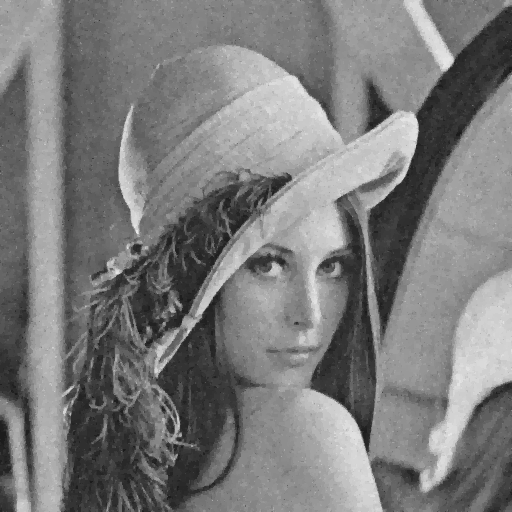
\includegraphics[scale=0.25]{Images/2_L1_20}
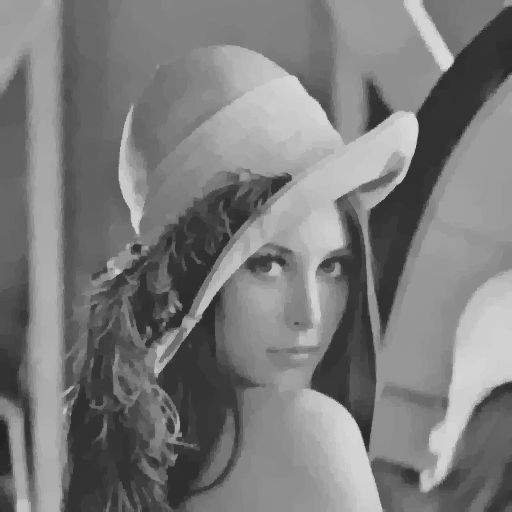
\includegraphics[scale=0.25]{Images/2_L1_50}
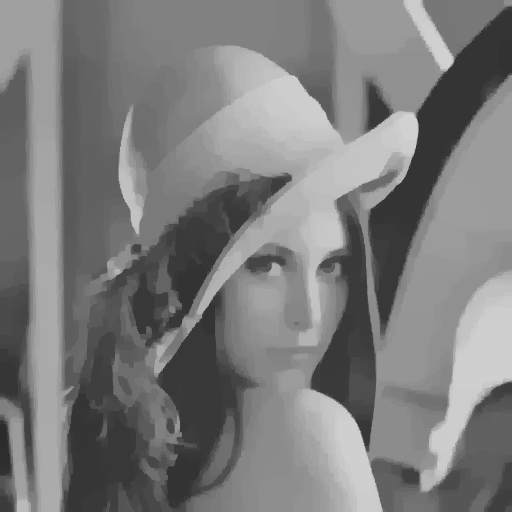
\includegraphics[scale=0.25]{Images/2_L1_100}
\hspace{10 pt}
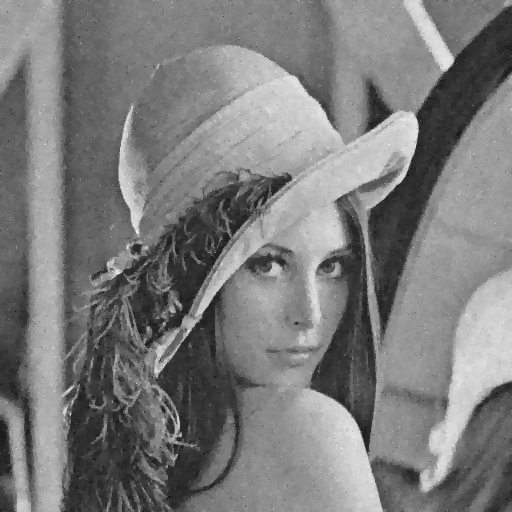
\includegraphics[scale=0.25]{Images/2_SEF_83_20}
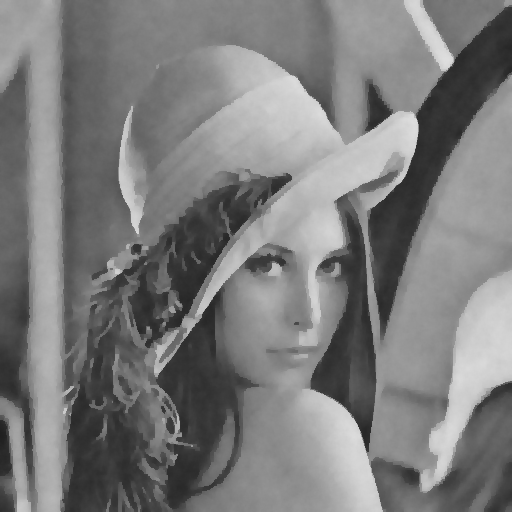
\includegraphics[scale=0.25]{Images/2_SEF_212_50}
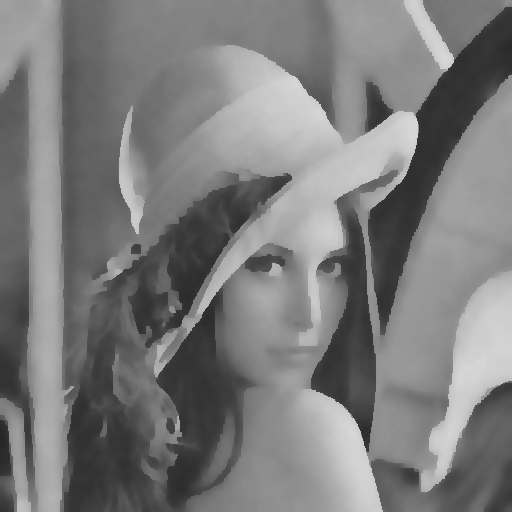
\includegraphics[scale=0.25]{Images/2_SEF_430_100}
\caption{Résultats de la remise à L’échelle de la régularisation. Sur la première ligne les solution par régularisation $L1$ pour les paramètre $\lambda=20$, $\lambda=50$, $\lambda=100$ et sur la deuxième ligne les résultats avec régularisation par la $SEF_{0.5,4}$. Les paramètres calculés sont $\lambda=83$, $\lambda=212$, $\lambda=430$. Visuellement l'intensité de la régularisation parait similaire dans les trois cas.}
\label{fig:L1_SEF}
\end{figure}

%Une autre alternative est de considérer dans le contexte bayésien, que la fonction de régularisation est le -log de la distribution, ainsi $h_2(x) = \frac{1}{N} e^{-g_2(x)}$ avec $N$ un paramètre de normalisation.
%\begin{equation}
%\hat{\lambda}_2 = \lambda_1 \frac{\sum_i{e^{-g_2(i)}} \sum_i{h_1(i)g_1(i)}}{\sum_i{g_2(i)e^{-g_2(i)}}}
%\end{equation}
%Cette approche suppose que le modèle $E_2$ est le "bon" modèle qui décrit correctement le problème.

\subsection{Comparaison entre Ishikawa et $\alpha$-Expansion}

Les méthodes d'optimisation par coupure de graphes sont applicables pour certaines catégories de fonctions de régularisation. Pour comparer les performances d'optimisation $\alpha$-Expansion avec le minimum global obtenu par le graphe d'Ishikawa, il faut que la fonction de régularisation soit gérée par les deux méthodes ce qui réduit grandement les possibilités de modèle. Nous nous plaçons dans dans cas : la norme L1 et la norme L1-lissée.

\subsubsection{Cas de la régularisation par la norme $L1$}
Nous nous plaçons dans le cas où la fonction de régularisation est la norme $L1$. L'hypothèse de la norme $L1$ correspond à une distribution de Laplace de l'écart entre pixel voisins. Le choix de cette loi est motivé par les contraintes des méthodes d'optimisation et n'est pas forcement la loi décrit le mieux les données. Le jeu test est composé de 5 images en niveau de gris. Les expérimentations sont réalisés pour trois bruits indépendants, un bruit gaussien d'écart-type $\sigma=20$, un bruit laplacien d'échelle $s=20$ et un bruit de Cauchy d'échelle $s=20$. Les valeurs en dehors de l’intervalle des données saturent aux valeurs extrêmes. La fonction de régularisation est  $g(x)=|x|$, les fonctions d'attache aux données pour les trois bruits sont $f(x)=x^2$, $f(x)=|x|$, $f(x)=ln(1+\frac{x^2}{s^2})$ et les facteur de régularisation sont $\lambda=0.8$, $\lambda=0.8$, $\lambda=0.04$. 

\begin{table}
\centering
\begin{tabular}{c|cc|cc|cc|cc}
 & \multicolumn{4}{c|}{Gauss $\sigma=20$}  & \multicolumn{4}{c}{Laplace $s=20$} \\
 & \multicolumn{2}{c|}{Ishikawa}  & \multicolumn{2}{c|}{$\alpha$-Expansion} & \multicolumn{2}{c|}{Ishikawa}  & \multicolumn{2}{c|}{$\alpha$-Expansion}  \\
Image & énergie & temps & énergie & temps & énergie & temps & énergie & temps \\
\hline
Pepper &  \num{13544952} & \SI{55,4}{s} & +\num{0} & \SI{10,3}{s} &  \num{12549064} & \SI{52,4}{s} & +\num{0} & \SI{9.40}{s}\\
Barbra & \num{56634892} & \SI{241}{s} & +\num{0} & \SI{40,5}{s} & \num{48279928} & \SI{231}{s} & +\num{0} & \SI{40,5}{s}\\
Boat & \num{51704102} & \SI{200}{s}    & +\num{0} & \SI{39.6}{s} & \num{51704102} & \SI{186}{s}    & +\num{0} & \SI{36.5}{s}\\
House & \num{12310902} & \SI{47,4}{s}    & +\num{0} & \SI{9.10}{s} & \num{11195042} & \SI{42.2}{s}    & +\num{0} & \SI{8.2}{s}\\
Lena & \num{48999864} & \SI{207}{s}    & +\num{0} & \SI{38.2}{s} & \num{44820374} & \SI{189}{s}    & +\num{0} & \SI{35.6}{s}\\
\end{tabular}
\caption{Comparaison entre $\alpha$-Expansion et Ishikawa de l'énergie finale et le temps d’exécution pour un bruit gaussien et un bruit laplacien. Dans l'expérimentation $\lambda=0.8$ et les énergies sont données à un facteur 10. On remarque que la solution $\alpha$-Expansion est une solution minimale du problème.}
\label{tab:denoise_exp_ish}
\end{table}

\begin{table}
\centering
\begin{tabular}{c|cc|cc|}
 & \multicolumn{4}{c|}{Cauchy $s=20$} \\
&  \multicolumn{2}{c|}{Ishikawa}  & \multicolumn{2}{c|}{$\alpha$-Expansion}   \\
Image & énergie & temps & énergie & temps \\
\hline
Pepper &  \num{6447042} & \SI{69,5}{s} & +\num{5} & \SI{18,4}{s}  \\
Barbra & \num{25462129} & \SI{276}{s} & +\num{19} & \SI{76,6}{s} \\
Boat & \num{24556292} & \SI{225}{s}    & +\num{3} & \SI{70.6}{s} \\
House & \num{5926775} & \SI{50,5}{s}    & +\num{5} & \SI{15.7}{s} \\
Lena & \num{23585990} & \SI{234}{s}    & +\num{29} & \SI{68.2}{s} \\
\end{tabular}
\caption{Comparaison entre $\alpha$-Expansion et Ishikawa de l'énergie finale et le temps d’exécution pour un bruit de Cauchy. Dans l'expérimentation $\lambda=0.04$ et les énergies sont données à un facteur 100. La solution $\alpha$-Expansion est n'est pas minimale en étant toutefois très proche du minimum global.}
\label{tab:denoise_exp_ish_2}
\end{table}

Les résultats pour les bruits gaussiens et laplacien sur les 5 images de la base de test sont donnés dans la Tab~\ref{tab:denoise_exp_ish}. En pratique $\alpha$-Expansion converge en deux itérations - la deuxième ne servant qu'à constater que la solution a convergé, la solution finale est optimale. Le temps d’exécution est envions 5 fois inférieur à celui du graphe d'Ishikawa. Ainsi, les sous-espaces explorés par $\alpha$-Expansion suffisent à atteindre le minimum global. Les résultats pour le bruit de Cauchy sont donnés dans la Tab~\ref{tab:denoise_exp_ish_2}. $\alpha$-Expansion converge en trois itérations mais n'atteint pas le minimum global d!e l'énergie. La valeur du minimum reste toutefois très proche (écart entre 3 et 29). A la différence des deux cas précédents, dans ce troisième cas le modèle n'est pas convexe. Il apparaît qu'$\alpha$-Expansion est susceptible d'atteindre rapidement le minimum global quand le modèle est convexe, mais que ces performances sont réduites pour des attaches aux données non-convexes.

\subsubsection{Cas de la régularisation par la "norme $L1$-lissée"}

Nous nous plaçons maintenant de la cas d'un bruit gaussien décrit précédemment avec le même modèle d'attache aux données. La fonction de régularisation est une "norme $L1$ lissée"  définie comme,
\begin{equation}
		\begin{aligned}
				g(x) = a|x| &, \; \text{si } |x| \leq 1 \\
				g(x) = b|x| &, \; \text{sinon}.
		\end{aligned}
\end{equation}
avec $a \leq b$. C'est une fonction convexe présentant une cuvette autour de zéro. En principe la fusion expansion ne peut pas être mise en œuvre pour avec cette fonction de régularisation. Cependant, comme la fonction est convexe, la fusion peut être optimisée globalement moyennant un changement de variable (voir Partie~\ref{sss:fus_conv}). Nous comparons trois approches : celle d'Ishikawa, $alpha$-expansion et un schéma alterné expansion et saut composé de l'ensemble des expansion et des saut +1 et -1. La structure du graphe d'Ishikawa étant très volumineuses, nous faisons les expérimentations sur des sous-image de taille 128 par 128.

\begin{table}
\centering
\begin{tabular}{c|cc|cc|cc}
\hline
\multirow{2}{*}{Méthode} & \multicolumn{2}{c|}{Pepper} & \multicolumn{2}{c|}{Barbra} & \multicolumn{2}{c}{Boat} \\ 
 & Énergie & temps & Énergie & temps & Énergie & temps  \\
\hline
Ishiwaka & \num{14336480} & \SI{335}{s} & \num{13017181
} & \SI{347}{s} &  \num{18077919} & \SI{338}{s}  \\
$\alpha$-Exp & +\num{251486} & \SI{10.6}{s} & +\num{202214} & \SI{11.7}{s} & +\num{179278} & \SI{10.5}{s}  \\
$\alpha$-Exp QPBO & +\num{134795} & \SI{23.3}{s} & +\num{126744} & \SI{20.6}{s} & +\num{112458} & \SI{22.0}{s} \\
$\alpha$-Exp QPBO-P & +\num{134795} & \SI{42.7}{s} & +\num{126744} & \SI{38.1}{s} & +\num{112458} &  \SI{38.9}{s} \\
$\alpha$-Exp Convexe & +\num{133659} & \SI{16.3}{s} & +\num{123607} & \SI{12.4}{s} & +\num{104454} & \SI{13.5}{s} \\
Saut $+1/-1$ & +\num{0} & \SI{2.75}{s} & +\num{0} & \SI{2.17}{s} & +\num{0} & \SI{2.80}{s} \\
\hline
\multirow{2}{*}{Méthode} & \multicolumn{2}{c|}{House} & \multicolumn{2}{c|}{Lena} \\ 
 & Énergie & temps & Énergie & temps  \\
\cline{1-5}
Ishiwaka & \num{14321340} & \SI{263}{s} & \num{12426375
} & \SI{278}{s} \\
$\alpha$-Exp relaxé & +\num{151920} & \SI{10.6}{s} & +\num{265218} & \SI{11.7}{s}  \\
$\alpha$-Exp QPBO & +\num{94446} & \SI{23.3}{s} & +\num{158157} & \SI{20.6}{s} \\
$\alpha$-Exp QPBO-P & +\num{94446} & \SI{42.7}{s} & +\num{158157} & \SI{38.1}{s}\\
$\alpha$-Exp Convexe & +\num{91732} & \SI{11.9}{s} & +\num{154346} & \SI{15.4}{s} \\
Saut $+1/-1$ & +\num{0} & \SI{2.53}{s} & +\num{0} & \SI{2.08}{s} \\
\end{tabular}
\caption{Comparaison des méthodes d'optimisation dans le cas d'une régularisation par la norme L1-lissée. Les valeurs d’énergie sont données par rapport au minimum global obtenu par le méthode Ishikawa. Les autres méthodes sont $\alpha$ expansion optimisé par fusion relaxée, QPBO, QPBO-P, reformulé en fusion convexe et enfin le schéma Saut composé de deux fusions : le Saut +1 et le Saut -1.}
\label{tab:L1_L2}
\end{table}

Le schéma $\alpha$-Expansion n'a pas été proposé dans le cas de fonction de régularisation métrique, or la fonction de régularisation utilisée est non-métrique. Il en résulte des sous-problèmes binaires non-sous-modulaires. 4 méthodes sont utilisées pour résoudre ces sous-problèmes : la relaxation, QPBO, QBPO-P et la réécriture en fusion convexe. Il apparaît que la convergence de la fusion relaxée est deux fois plus rapide que QPBO, il-même deux fois plus rapide que QPBO-P. Les minima de QPBO et QPBO-P sont égaux et inférieurs au minimum de la fusion relaxée, et très proche du minimum obtenu par résolution exacte (fusion convexe). Toutefois, la fusion convexe ne permet pas d'atteindre le minimum global. La schéma par Saut converge vers le minimum global, cela s'explique par le fait que ce schéma d'optimisation d'apparente à une descente de gradient et que dans le cas d'une énergie convexe, cette méthode converge vers le minimum global. Il ressort de ce résultat que s'il est possible que traiter des régularisations convexe avec $\alpha$-Expansion, ce sch"ma d'optimisation n'est pas adaptée à la norme $L1$-lissée.

\subsection{Comparaison des performances des différents schémas d'optimisation}

Dans cette partie la fonction de régularisation est obtenue en observant l'histogramme des écarts de valeur entre voisin. La forme de la fonction $g$ est déterminée par le -log de l'histogramme. 
\begin{equation}
E(\boldsymbol{l}) = \sum_{i \in \boldsymbol{I}}{ (l^b_i - l_i)^2} + 
\lambda \sum_{(i,j) \in \boldsymbol{N'}}{ SEF_{a,s}(l_i-l_j) }
\end{equation}
où $SEF_{a,s}$ est une fonction exponentielle lissée (\ref{eq:def_SEF}). Pour $a=2$, $SEF$ est une fonction quadratique. Ces fonctions ont la particularité d'être une approximation quadratique autour de zéro et une puissance pour de grandes valeurs, elle correspond au moins $-\text{log}$ d'une distribution proche d'une gaussienne autour de zéro et d'une autre loi pour de grandes valeurs. $a=2$ correspond à une distribution gaussienne, $a=1$ à une distribution de Laplace lissée et pour $a \rightarrow 0$ à une distribution de Cauchy. Pour des valeur de $a$ inférieures à $1$ la fonction est ni convexe et ni concave sur $\mathbb{R}^+$, les problèmes de fusion sont donc non-sous-modulaires et des méthodes approchées doivent être mise en œuvre. Dans cette partie nous prendrons $f(x)=x^2$, $g(x)=SEF_{0.5,4}$ et $\lambda=100$. Nous prenons en compte 4 schéma d'optimisation, soit $[-T, T]$ l'intervalle où la régularisation est convexe,
\begin{itemize}
\item $\alpha$-Expansion
\item Alterné-C : schéma alterné complet avec toutes des expansions et toutes les sauts.
\item Alterné-L : schéma alterné avec toutes des expansions et les sauts limité dans l'intervalle $[-T, T]$.
\item Alterné-LQ : schéma alterné avec les expansions à intervalle $T$ et les sauts limités dans l'intervalle $[-T, T]$.
\end{itemize}

\subsubsection{Comparaison entre les schémas d'optimisation}

	Le schéma d'optimisation Alterné-C est une extension d'$alpha$-Expansion. Il est composé de toutes les expansions et de tous les sauts possibles. Cela a deux conséquences : 1) l'espace des solutions explorées est plus grand, 2) le temps d'exécution d'un cycle du schéma est plus important. Il peut en résulter une énergie plus basse dans un temps plus important. Cependant, l’énergie possède de nombreux minima locaux qui peuvent empêcher une descente de l’énergie et le surcout en temps de chaque cycle peut être compensé par un nombre de cycle réduit. Nous avons testé 3 méthodes d'optimisation pour résoudre les sous-problème de fusion : la fusion relaxée, $QPBO$ et $QPBO{-}P$. Les résultats pour les 5 images de la base de test sont donnés dans la première partie de la Table~\ref{tab:schema_comp}. L'introduction des fusions saut permet de faire baisser l’énergie substantiellement (de l'ordre 2\% de l’énergie) quelque soit la méthode d'optimisation. Cela entraîne un surcoût en temps de calcul assez important pour la fusion relaxée (d'un facteur 2 à 3), plus réduit pour les méthodes QPBO et QPBO-P (de +5\% à +40\%) le temps supplémentaire par cycle étant en partie compensé par un nombre de cycle plus réduit. Les temps d’exécutions des méthodes QPBO et QPBO-P restent supérieurs à ceux de la fusion relaxée. En conclusion, le schéma $alpha$-Expansion n'est pas adapté au problème où la fonction de régularisation possède une cuvette convexe autour de zéro, même employant des méthodes d'optimisation plus optimales.
		
\begin{table}
\centering
\begin{tabular}{c|cc|cc|cc}
& \multicolumn{2}{c|}{Fusion relaxée} & \multicolumn{2}{c|}{QPBO} & \multicolumn{2}{c}{QPBO-P} \\
 & $\Delta$E & $\tau$t & $\Delta$E & $\tau$t & $\Delta$E & $\tau$t  \\
\hline
Image & \multicolumn{6}{c}{$\alpha$-Expansion} \\
\hline
Pepper & \num{783004 } &	20\% &	\num{184831} &	50\% &	\num{184501} &	88\% \\
Barbra & \num{2779150} &	12\% &	\num{709860} &	36\% &	\num{709302} &	62\% \\
Boat & \num{2938868} &	21\% &	\num{743708} &	47\% &	\num{743499} & 81\%	 \\
House & \num{742441 } &	22\% &	\num{194914} &	56\% &	\num{194884} &	95\% \\
Lena & \num{3133824} &	15\% &	\num{764929} &	45\% &	\num{764497} &	75\% \\
\hline
Image & \multicolumn{6}{c}{Alterné-C} \\
\hline					
Pepper & \num{1111} &	39\% &	6	& 59\% &	0 &	100\%   \\
Barbra & \num{5602} &	36\% &	40	& 50\% &	0 &	100\%   \\
Boat & \num{4025} &	42\% &	128	& 60\% &	0 &	100\%   \\
House & \num{606 } &	49\% &	-34	& 58\% &	0 &	100\%   \\
Lena & \num{3662} &	30\% &	68	& 59\% &	0 &	100\%   \\
\hline
Image & \multicolumn{6}{c}{Alterné-L} \\
\hline					
Pepper & \num{1177} & 14\% &   \num{205 } & 22\%  &  \num{177 } & 37\%   \\
Barbra  & \num{5815} & 69\% &   \num{224 } & 164\%  &  \num{297 } & 236\%  \\
Boat & \num{4190} & 78\% &   \num{192 } & 103\%  &  \num{126 } & 153\%  \\
House & \num{659 } & 15\% &   \num{-21 } & 18\%  &  \num{1   } & 31\%   \\
Lena & \num{3761} & 62\% &   \num{160 } & 89\%  &  \num{97  }  & 171\%  \\
\hline
Image & \multicolumn{6}{c}{Alterné-LQ} \\
\hline					
Pepper & \num{1183} & 7\% &   \num{225 } & 10 \%   &  \num{217 }  & 17\%   \\
Barbra & \num{5393} & 25\% &   \num{-232} & 50\%  &  \num{-245} & 85\%   \\
Boat & \num{3598} & 25\% &   \num{323 } & 37\%  &  \num{310 } & 62\%   \\
House & \num{693 } & 5\% &   \num{88  } & 8  \%   &  \num{83  } & 14\%   \\
Lena & \num{3586} & 26\% &   \num{85  } & 36\%  &  \num{67  } & 61\%   \\
\end{tabular}
\caption{Comparaison entre les schémas d'optimisation $\alpha$-Expansion et Alterné-C pour trois méthodes d'optimisation. Les valeurs d’énergie sont données en écart à l’énergie QPBO-P pour le schéma Alterné-C, les temps d’exécution sont données en pourcentage du temps d’exécution de QPBO-P pour le schéma Alterné-C.}
\label{tab:schema_comp}
\end{table}

	Les schémas Alterné-L et Alterné-QL sont analogues à Alterné-L avec un ensemble de fusion par cycle restreint. Les résultats de ces deux schéma sont donnés dans la dernière partie de la Table~\ref{tab:schema_comp}. Nous remarquons dans les énergies sont très proches pour des trois schémas. Le schéma Alterné-C donne la meilleure énergie sauf pour l'image "Barbra". Les temps d’exécutions du schéma Alterné-L peut aussi bien réduire de moitié comme doubler du fait d'un nombre de cycle nécessaire à la convergence plus important. Les temps de convergence d'Alterné-QL sont inférieurs à ceux des deux autres schémas. En conclusion, les trois schémas sont adaptés au problème. Le schéma Alterné-C donne généralement la meilleur énergie. Le schéma Alterné-L donne une énergie un peu supérieure et son temps d’exécution peut être important. Le schéma Alterné-LQ permet un gain important en temps d'exécution en impactant très peu l’énergie finale.

\subsubsection{Comparaison des temps de convergence des différents schémas}

Dans la \ref{tab:schema_comp}, il apparaît que le temps de convergence de QPBO-P est supérieur à celui de QPBO pour des performance très proches en terme d’énergie. La fusion relaxée converge plus rapidement  que les méthodes QPBO.

Si le temps de convergence est très long, il est très fréquent que les derniers cycles les derniers cycles des schémas n'optimisent que très peu la solution. En pratique il est courant d’arrêter les itérations de manière anticipée et les conclusions sur les performances respectives des méthodes peuvent changer. La Figure~\ref{fig:comp_opt__} représente l'évolution de l’énergie au cours du temps. Les images 5 images sont regroupées en deux graphiques en fonction de leur taille. Le comportement de QPBO et QPBO-P sont très proches, si ce n'est que le temps d’exécution est plus lent pour QPBO-P. La fusion relaxée permet une décroissance de l’énergie moins rapide à chque cycle mais est exécutée plus rapidement. Elle converge vers une solution d’énergie supérieure à celles obtenues par les méthodes QPBO.

\begin{figure}
\centering
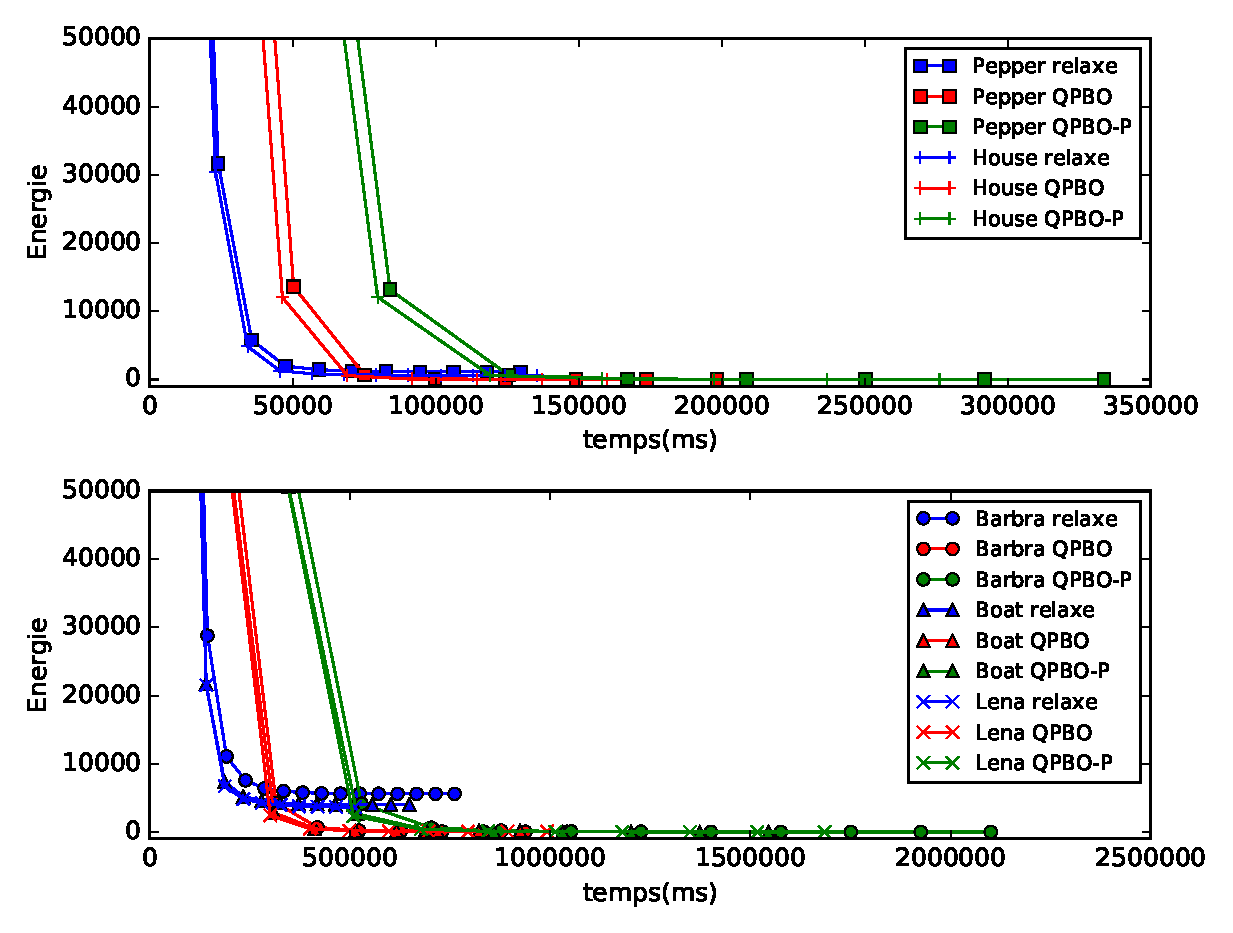
\includegraphics[scale=0.75]{Data/Opt_Comp}
\caption{Évolution de l’énergie au cours du temps pour les trois méthodes d'optimisation sur la base de test dans le cas du schéma d'optimisation ALterné-C. Les énergies sont données à une constante près et seul la première itération ne chaque méthode est en dehors du graphe.}
\label{fig:comp_opt__}
\end{figure}

\section{Conclusion}

	Les problèmes multi-label sont des problèmes difficiles. La décomposition d'un problème multi-label en sous-problème binaire permet d'obtenir des solutions approchées. Chaque sous-solution permet de diminuer l’énergie de la solution courante. Cette méthode demande d'explorer de manière efficace l'espace des solutions selon un schéma d'optimisation. Nous avons proposé un schéma d'optimisation dans le cas des fonctions convexes autour de zéros et concave pour de grandes valeurs qui alterne fusion Expansion et Saut, Alterné-C et ses variantes Alterné-L et Alterné-LQ. L’intérêt de ce schéma par rapport à des schémas plus classiques telles qu'$\alpha$-Expansion est illustré sur le problème de dé-bruitage. Dans le cas d'un modèle convexe $\alpha$-Expansion atteint dans la pratique le minimum global, toutefois la modalisation statistique du problème amène à optimiser des fonctions telles que décrites précédemment et pour lesquelles $\alpha$-Expansion n'est pas suffisant. Les variantes Alterné-L et Alterné-LQ permettent de converger plus rapidement vers une énergie légèrement plus élevée. En outre, nous avons comparé l'utilisation de plusieurs méthodes d'optimisation des fusions binaires. La fusion relaxée est la plus rapide, mais optimise moins bien que la méthode QPBO. L'apport de la méthode QPBO-P est très limité. Toutefois ces conclusions sont à nuancer. En effet, le problème de dé-bruitage est relativement simple puisque les attaches aux données sont des fonctions monotoniques, ce qui limite le nombre de minimum local. Dans le cas d'attache aux données plus complexe, les méthodes approchées pourraient être mises en défaut.

%\bibliographystyle{unsrt}
\bibliographystyle{apalike-fr}
\bibliography{../bibliography/Bib_1}

%----------------------------------------------------------------------------------------
\end{document}
%----------------------------------------------------------------------------------------
